\documentclass[12pt]{article} % Default font size of the document, change to 10pt to fit more text

\usepackage{newcent} % Default font is the New Century Schoolbook PostScript font 
%\usepackage{helvet} % Uncomment this (while commenting the above line) to use the Helvetica font

\usepackage[utf8]{inputenc}
\usepackage[francais]{babel}
\usepackage[T1]{fontenc}

% Reference the bibliography in summary
\usepackage[nottoc,notlof,numbib]{tocbibind}

% Graphics preamble
\usepackage{graphicx} % Allows to import images
\usepackage{float} % Allows for control of float positions

\usepackage[margin=1.4in,includefoot]{geometry}

\begin{document}

\begin{titlepage}
	\begin{center}
	\line(1,0){400} \\
	[0.25in]
	\huge{\bfseries Analyse d'un Carrefour} \\
	[2mm]
	\line(1,0){300} \\
	[1.5cm]
	\textsc{\LARGE UV 5.8 Ingénierie Systèmes} \\
	[0.75cm]
	\textsc{\Large Bureau d'études – Simulation} \\
	[10cm]
	\end{center}
	\begin{flushright}
	\textsc{\large Evandro Bernardes \\ Mohamed Shehade \\ Sergio Pertierre do Monte  \\}
	\end{flushright}

\end{titlepage}

% Table of contents
\tableofcontents
\thispagestyle{empty}
\cleardoublepage


% List of figures, list of tables
\listoffigures
\cleardoublepage

\setcounter{page}{1}

\section{Objectif de l'étude}\label{sec:1}
La présente étude a comme but trouver une solution qui améliore le trafic d'un quartier de la ville de Brest qui pâtit des embouteillages.

\begin{figure}[H]
	\centering
	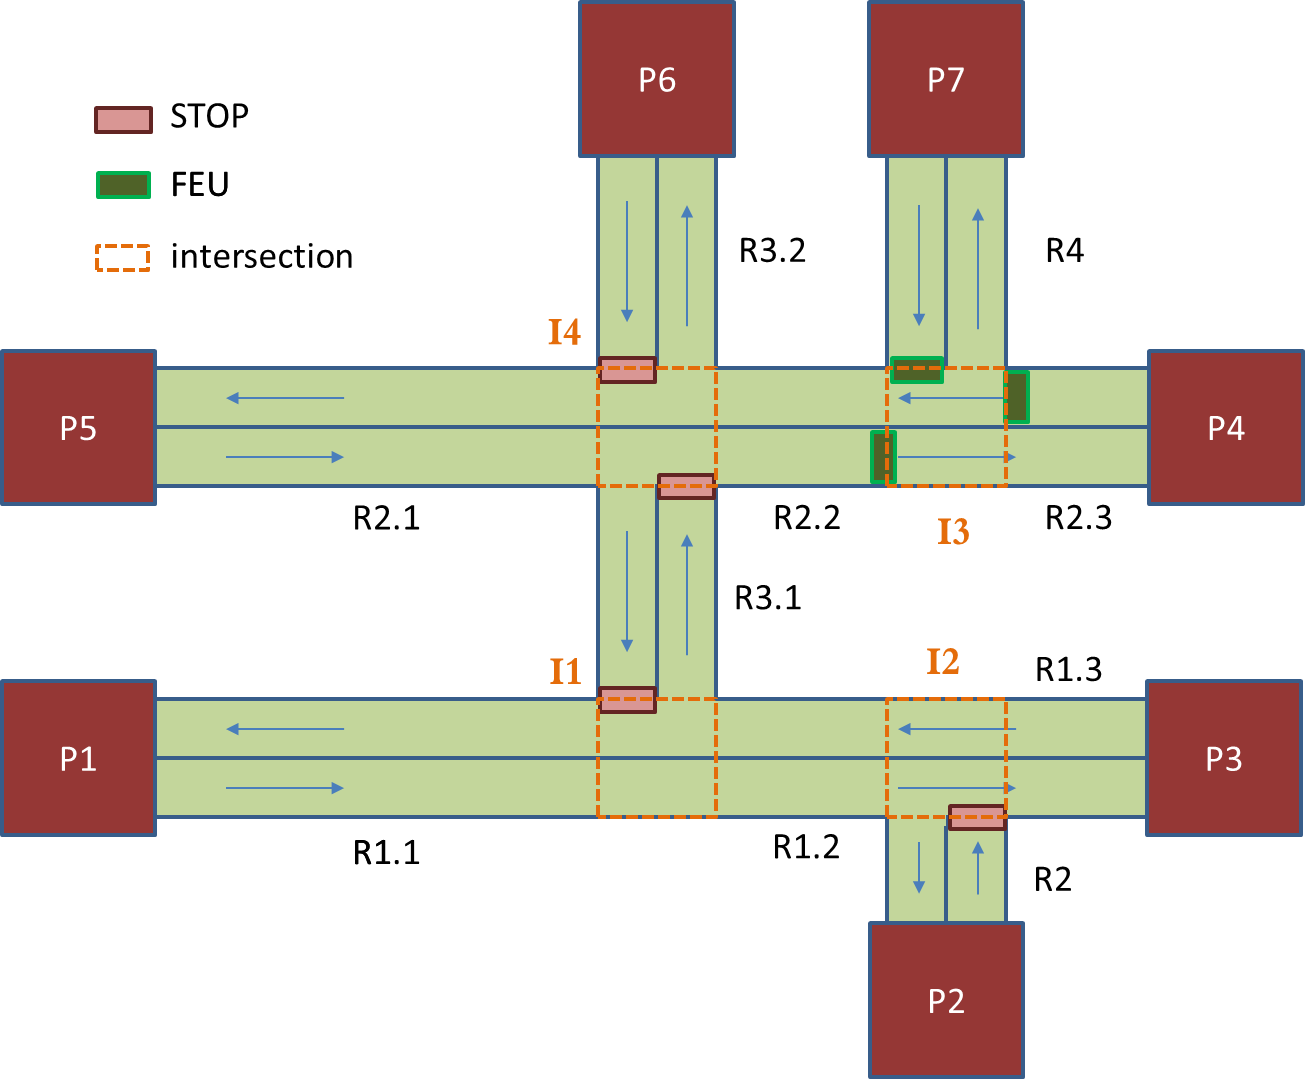
\includegraphics[width=\linewidth]{Figure1.png}
	\caption{Carrefour Routier de Coruscant}
	\label{fig:fig1}
\end{figure}

Le maire de Brest, M Remai, souhaite améliorer le trafic dans le grand carrefour routier « Coruscant » suite à plusieurs plaintes apportées par les usagers de ce quartier à cause de nombreux embouteillages. Donc, M Remai a demandé à la société TrafBreizh de faire une étude de l'évolution du quartier pour y trouver des solutions.

D’ailleurs, étant donné que cette situation existe en autres zones, le maire a mis plusieurs tranches optionnelles dépendant de la réussite de cette première tranche.

L'entreprise TrafBreizh a comme objectif développer un outil efficace qui puisse résoudre le problème et qui soit capable de s'adapter à d'autres problèmes futures.

Donc, d'abord, pour trouver la solution de cette tâche, en utilisant un moteur de simulation on cherche recréer l'environnent du quartier avec les données fournies qui montrent les caractéristiques des différentes parties élémentaires pertinentes à l'analyse du problème, telles comme les zones d'accès au carrefour et ses routes, l'accélération et la longueur des véhicules, le fonctionnement des feux.

Aussi, pour faciliter cette simulation on a adopté quelques hypothèses pour les voitures comme sera montré ultérieurement, par exemple, elles ont la même taille et suivent les lois de circulation française.

Donc, après avoir obtenu les résultats, on a changé plusieurs paramètres de la simulation en utilisant les exigences du client pour obtenir une solution optimale.
\newpage
\section{Analyse du problème}\label{sec:2}
Plusieurs sous-systèmes doivent être implémentés pour l’implémentation de cette simulation. Un système qui crée tout l’environnement au démarrage et qui démarre le moteur de simulation. Aussi un système qui calcule le chemin à être suivi selon les endroits de départ et d’arrivée de chaque voiture, et un système de création de voitures. 

\subsection{Environnement et variables d'état}
L’environnement compte avec plusieurs entités. Les principales sont : 

\begin{itemize}
\item \textbf{Véhicules :}
Une entité modélisant les véhicules. Chaque voiture doit avoir des variables comme : vitesse, lieux de départ et arrivée, position actuelle, route actuelle, une référence qui indique la voiture qui est juste devant et des variables booléens indiquant quelques états : si la voiture est déjà arrivée, si elle est en train d’attendre le feu vert, si elle est bloquée par une voiture qui est devant.

\begin{figure}[H]
	\centering
	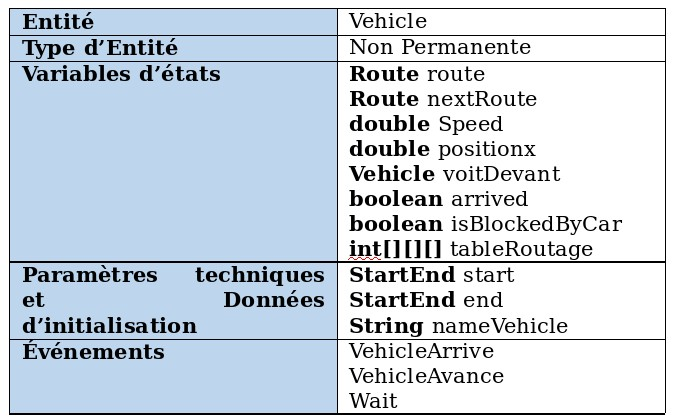
\includegraphics[width=\linewidth]{Vehicle.png}
	\caption{Classe « Vehicle »}
	\label{fig:Vehicle}
\end{figure}

\item \textbf{Routes :}
Une classe pour modéliser les routes. Elle doit être munie d’une liste des voitures actuellement présentes, des intersections, les endroits de début et de fin, le nom de la route.

\begin{figure}[H]
	\centering
	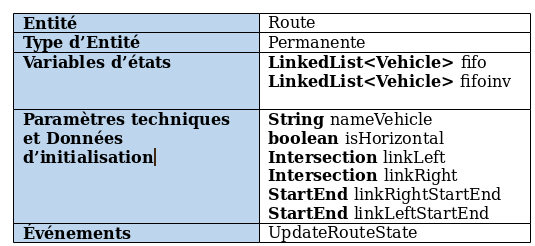
\includegraphics[width=\linewidth]{Route.png}
	\caption{Classe « Route »}
	\label{fig:Route}
\end{figure}

\item \textbf{Start / End :}
Classe qui décrit où sont les points d'entrée et sortie du quartier.

\begin{figure}[H]
	\centering
	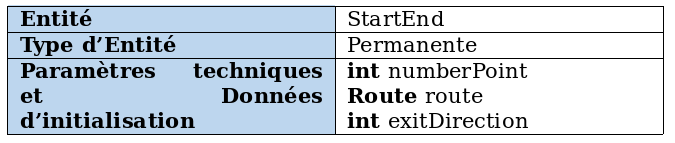
\includegraphics[width=\linewidth]{StartEnd.png}
	\caption{Classe « StartEnd »}
	\label{fig:StartEnd}
\end{figure}

\item \textbf{Intersections :}
Cette classe doit contenir des références vers les routes qu’elle connecte, des références vers les voitures qui attendent sur chaque route connectée. Aussi faut-il créer un système pour bien implémenter le type d’intersection : Combien de routes elle connecte, s’il y a des feux ou pas. 

\begin{figure}[H]
	\centering
-	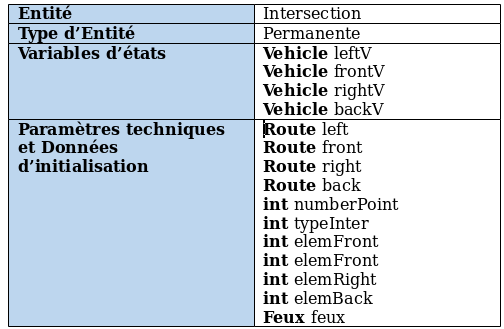
\includegraphics[width=\linewidth]{Intersection.png}
	\caption{Classe « Intersection »}
	\label{fig:Intersection}
\end{figure}

\end{itemize}

\subsection{Liste des évènements}
En plus, il faut implémenter les événements importants de la simulation : 

\begin{itemize}
\item La création d'un objet véhicule (simulant l'arrivée d'une voiture dans le quartier) ;\\

\item Le passage des feux vert ;\\

\item Quand il faut qu'une voiture s'arrête pour attendre les feux ;\\

\item Un événements de mise à jour des entités (routes, voitures, etc...).
\end{itemize}
%\subsection{Hypothèses particulières}

\begin{figure}[H]
	\centering
	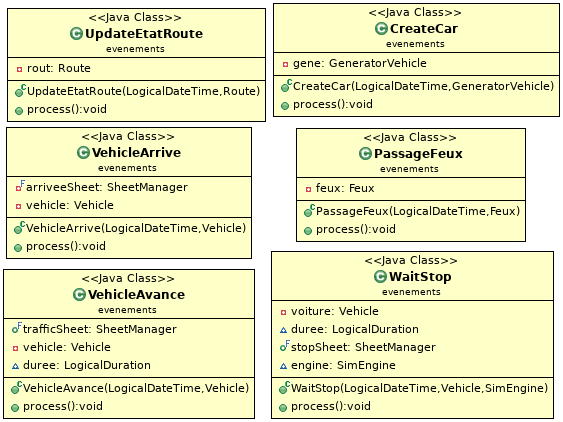
\includegraphics[width=0.9\linewidth]{UML_evenements.png}
	\caption{Les événements.}
	\label{fig:UML_evenements}
\end{figure}

\newpage
\section{Modélisation du système}\label{modelisation}
Pour modéliser un quartier comme Coruscant dans le système de simulation, il faut d'abord bien définir les lois que suivront chaque entité. C'est-à-dire : il faut qu'on modélise bien chaque action de la voiture dans chaque circonstance, selon les variables d'états des autres entités comme les routes et les intersections. Bien évidemment, ces variables seront elles aussi gérées par des lois de comportement décrivant chaque instance de ces entités permanentes qui composent le quartier étudié.
%
\subsection{Routes}
Les routes doivent à chaque itération compter le nombre de véhicules qui elles comportent. Elles doivent toujours mettre à jour ses listes en vérifiant quelles sont les voitures en train de passer.

\subsection{Intersections}
Les intersections effectuent toujours les « transactions » de voitures à travers les routes. Pour chaque voiture qui arrive à l'intersection, elle doit aussi recevoir la prochaine route sur laquelle la voiture veut passer. L'intersection doit vérifier si la voiture est sur une route verticale ou horizontale pour savoir quelle est la référence qui doit être libre. Pour finir, l'entité intersection ajoute le véhicule dans la liste de la nouvelle route et mets à jour quelques variables d'état importantes des véhicules :
\begin{itemize}
\item \textbf{route}, pour que l'objet voiture mette à jour son information de « route actuelle » ;\\

\item \textbf{sens}, pour montrer à quel sens roule la voiture ;\\

\item \textbf{position}, la localisation de la voiture sur la nouvelle route (0 ou la longueur de la route, parce que la valeur initiale de cette variable dépend du bout par lequel la voiture arrive) ;\\

\item \textbf{hasToStop}, on met la valeur « false » parce que la voiture ne doit plus attendre pour passer (elle l'a déjà fait).
\end{itemize} 

\subsection{Véhicules}
Les voitures sont les entités plus complexes à être modélisés. 
%
D'abord, l'information de quelles sont les routes par lesquelles la voiture doit passer sont calculées. Un boucle est créé pour calculer le chemin est les routes sont sauvegardés (en ordre) dans une liste.

Le moteur de simulation fait que les voitures suivent leur règles de comportement, comme :
\begin{itemize}
\item Régler la vitesse des voitures. Si on arrive à une intersection/feux, on doit diminuer la vitesse au cas où. Si on a une voiture devant nous, on ne peut pas avoir une vitesse plus haute que la sienne. ;\\

\item Vérifier si elle est bloquée par une voiture qui est devant (booléen « isBlockedByCar » de la classe Véhicule) ;\\

\item Vérifier s'il faut attendre à l'intersection et bien vérifier quand est-ce que la voiture peut passer (attendre les feux par exemple, s'il y a des feux dans l'intersection) ;\\

\item Bouger le véhicule sur la route selon sa vitesse.
\end{itemize} 

\subsection{Diagrammes de classes des entités}
\begin{figure}[H]
	\centering
	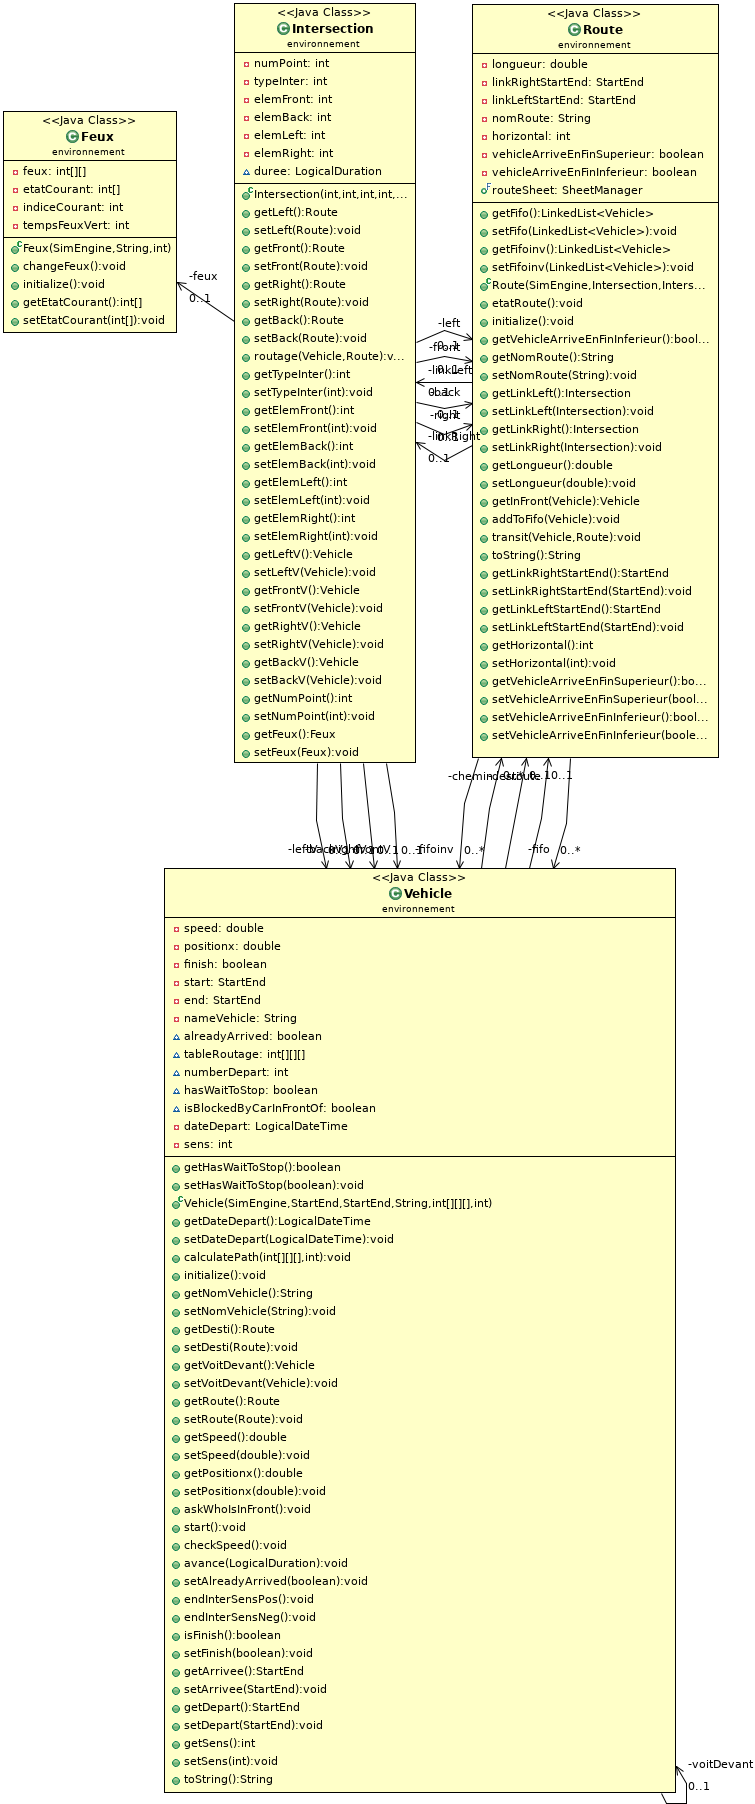
\includegraphics[height=0.9\textheight]{UML_entites.png}
	\caption{Relations entre les entités.}
	\label{fig:UML_entites}
\end{figure}

\newpage
\section{Implémentation du modèle}\label{implementation}
Le logiciel implémente des classes décrites dans quelques paquets de code Java. Les paquets utilisés sont le paquet « core » et le paquet « components », implémentant un système robuste et versatile de simulation qui peut être utilisé pour la création de plusieurs types d’environnement réels.

\subsection{Paquets du moteur de simulation :}
Le cœur du moteur de simulation, implémente (entre autres) les classes suivantes :

\begin{itemize}
\item \textbf{SimEngine :}
La classe SimEngine est la classe principale qui crée le moteur de simulation. Elle dépend de la graine générant les numéros aléatoires, entre autres paramètres.

En plus, dans cette classe il y a un système de notification (un « Listener ») qui notifie tout changement d'état du moteur. 

Après la mise en place du moteur de simulations avec les paramètres desquels il dépend, la simulation doit être lancé en exécutant une méthode d'initialisation, qui crée les événements et les objets pour toute la durée choisie de la simulation.

\item \textbf{SimObject :} Cette classe abstraite joue le rôle de l’entité manipulé le moteur de simulation, et doit connaître qui est le moteur de simulation qui doit l'animer.
Un SimObject a un nom et un identifiant unique, et peut être activé ou désactivé.\\

\item \textbf{SimTimeEvent :} Classe modélisant un événement temporel.\\

\item \textbf{SimEntity :} Hérite de SimObject, cette entité de simulation apporte de nouveaux services, comme des constructeurs utilisant les paramètres de l’entité, une gestion d’entités filles, et une gestion du cycle de vie de l’entité. Des Listeners permettent de notifier les changements d’état du système.
\end{itemize} 

\begin{figure}
	\centering
	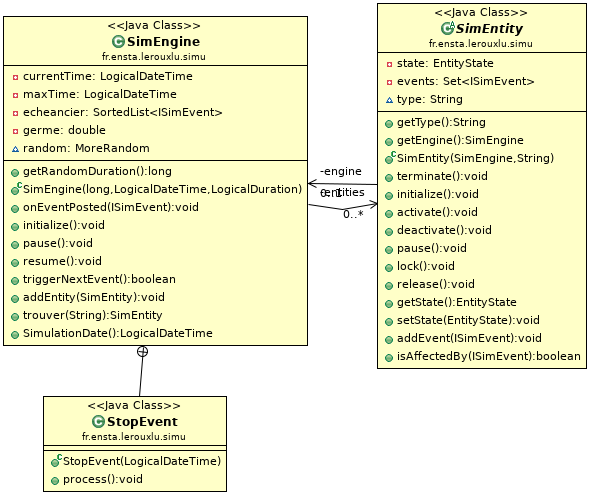
\includegraphics[width=0.9\linewidth]{UML_moteur.png}
	\caption{Les composants du moteur de simulation.}
	\label{fig:UML_moteur}
\end{figure}

\subsection{Système implémenté}
Le système implémente une classe « Monitor » qui joue le rôle de la méthode principale. Elle initialise deux loggers, un pour la sortie standard qui montre l'état après chaque événement et un autre qui crée un fichier dans lequel les résultats de la simulation seront sauvegardés. Pour le deuxième, le Monitor doit savoir où créer le fichier.

Suivant l'initialisation des loggers, le Monitor initialise le moteur de simulation, dont l'heure initiale et la durée de la simulation sont données comme paramètres. 

La troisième partie est la création de l'environnement. Le logiciel prend un fichier csv qui décrit la simulation, c'est-à-dire, quels intersections auront des feux et quels intersections sont simples. Le fichier possède ces informations en forme d'une variable binaire pour chaque intersection (1 si intersection simple, 2 si intersection avec des feux).
%
Ces paramètres sont utilisés dans le constructeur de la classe CreationEnvironnement, qui crée tous les entités de la simulation : les routes et les intersections (les informations pour la création des routes sont codes dans la classe CreationEnvironnement pour simplicité. Si jamais on veut réutiliser le même code pour un quartier différent, soit les routes/intersections doivent être changées pour décrire le nouvel environnement, soit ces informations doivent être inclues dans le fichier de paramètres (et la méthode doit être capable de lire ces informations, bien évidemment).
%
Cet objet environnement possède trois listes :
\begin{itemize}
\item \textbf{private LinkedList<StartEnd> listeStartEnd} : Pour savoir quels sont les points possibles d'arrivée et départ (objet StartEnd) ;\\

\item \textbf{private LinkedList<Intersection> listeInter} : Les intersections ;\\

\item \textbf{private LinkedList<Route> listeRoute} : Pour sauvegarder les routes crées par le constructeur.
\end{itemize} 

Pour finir, le Monitor lance la simulation, attend qu'elle finisse et ferme le logger créant le fichier des résultats.

\newpage
\section{Compte-rendu de V\&V}\label{VV}
\subsection{Introduction}

La vérification et validation (V\&V) sont importantes pour chaque étape de la construction du code. Avec les tests on peut trouver les erreurs du logiciel et les défauts du système concertant aux objectifs attendus dans son cycle de vie (en notre cas, plutôt la partie de conception et construction). Donc, la façon comment les tests étaient effectués et leur analyse sera présentée et détaillée ci-dessous.

D'abord, lors de l'analyse de besoins, on a définie les intentions à travers  des spécifications fonctionnelles, c'est-à-dire la façon dont les exigences seront prises en compte. Cette partie est important comme un guide pour que l'on ne s'éloigne pas des consignes et sert comme un prélude pour l'application des tests de V\&V.

Dans la vérification on peut noter la conformité avec les spécifications fonctionnelles établies dans les phases précédents du développement. Donc on cherche vérifier si le projet est conforme sa spécification et si l'on le fait de la manière correcte.

Finalement, dans l'étape de validation on produit de tests d'acceptation en se basant sur le cahier de charges. Le logiciel doit faire ce que l'utilisateur a besoin, alors on se focalise aux erreurs de concept relatifs à les exigences.
%==========================================================================
%verification :
%-faisons-nous le produit correctement [le projet doit etre conforme a sa specification]
%-erreurs par rapport aux définitions précises établies 

%validation :
%-Dans la partie de validation on se demande "faisons-nous le bon produit ?" [le logiciel doit faire ce que l'utilisateur a besoin]
%-Defaut par rapport aux besoin du client 
%====================================================================

\subsection{Processus}
Si l'on fait un rappel des exigences du client, il faut produire un outil capable de simuler une situation réel et que l'on puisse la modifier pour chercher des solutions et l'adapter à d'autres situations. Donc, le développement de tel outil demande de la rigueur, de l'abstraction et des connaissances approfondies en programmation.

Donc, vue que l'on a pris un code de base pour effectuer nos tests, plutôt qu'analyser le code en cherchant des erreurs (type statique de validation), on est centré dans l'exécution du même (type dynamique), i.e. on fait une analyse \textit{a posteriori} du système.

Puisque la priorité c'est de recréer l'ambiance réel du quartier de Coruscant pour que l'on puisse l'étudier, on a fait plusieurs tests pour corriger des erreurs et un test de validation pour examiner si les résultats correspondent au modèle donné :

\textsc{\Large DEMONSTRAçAO QUE A SIULAçAO CORRESPONDE AO MODELO DADO[MODELO CLASSICO]}

Il est possible de voir qu'il n'y a pas de défauts, donc on peut en déduire que le système est utilisable en pratique.

\textsc{\Large [MODELO ADAPTADO(soluçao)]}

\newpage
\section{Analyse des résultats de la simulation}\label{resultats}
This is

\newpage
\section{Perspectives d'évolutions}\label{evolution}
Pour qu’un meilleur logiciel de simulation puisse être implémenté, plusieurs modifications peuvent être envisagées : 

\begin{itemize}
\item Les voitures ne sont pas toutes identiques, c’est-à-dire, des modèles probabilistes peuvent être développées pour les paramètres décrivant les voitures ;\\

\item La création d’un modèle plus réaliste pour le redémarrage de la voiture ;\\

\item Trouver une manière de modéliser les événements particuliers (véhicule qui passe devant celui d’avant, par exemple) ;\\

\item Changer la méthode d'initialisation du système pour que les routes/intersections puissent aussi être facilement créées pour simuler d'autres quartiers ;\\

\item Ajouter une option pour étudier comment un accident ou une obstruction sur une de routes peut impacter les autres.
\end{itemize} 

\newpage
\bibliographystyle{plain}
\bibliography{bibfile}
\nocite{*}


\end{document}
